\documentclass[a4paper,12pt]{article}


\usepackage{minted}
\usepackage[cm]{fullpage}
%\usepackage[a4paper,margin=1in]{geometry}
\usepackage{graphicx}
\usepackage{amsmath}
\usepackage{capt-of}

\setminted[C]{fontsize=\small, tabsize=4, breaklines, linenos}
\setminted[Ruby]{fontsize=\small, tabsize=4, breaklines, linenos}
\setminted[text]{fontsize=\small, tabsize=4, breaklines, linenos}

%\setlength\parindent{0pt}

\title{Assignment 1 Report}
\author{Julius Putra Tanu Setiaji (A0149787E), Chen Shaowei (A0110560Y)}
\date{24 October 2018}

\begin{document}
\maketitle

\section{Program Design}
This train simulation is implemented in OpenMPI. Primary design considerations are:
\begin{itemize}
	\item Each edge is simulated by one process as required in the specifications.
	\item There is a master process responsible for the following:
	      \begin{itemize}
		      \item Distribution of information (map, lines) to slave processes.
		      \item Keeping track of train states (travelling/stationary).
		      \item Keeping track of station door open/close times.
		      \item Synchronising time across all slaves.
	      \end{itemize}
	\item Slave processes hold queues of trains and send them to each other, and reports to master whenever train states change.
\end{itemize}

\subsection*{Assumptions}

\begin{itemize}
	\item Only one train can open its doors at each station at any one time, regardless of direction.
	\item Train stations have infinite capacity for waiting trains.
	\item Time units are discrete and can have no subdivisions
	      \begin{itemize}
		      \item \textbf{Implication}: It is sufficient to store all time units as integers instead of floating point numbers
	      \end{itemize}
	\item Trains must open their doors for at least 1 unit of time.
	      \begin{itemize}
		      \item \textbf{Implication}: We round every randomly generated door open time up to the nearest integer
	      \end{itemize}
\end{itemize}

\section{Points to Note / Implementation Details}
\begin{itemize}
	\item Current simulation time needs to be shared across all processes. In addition, time can only be advanced after all processes have completed the actions to be done in the current tick.
	      \begin{itemize}
		      \item \textbf{Implication}: Explicit synchronisation messages need to be sent between master and slaves before and after the advancement of time.
	      \end{itemize}
	\item Each slave process maintains two queues of trains. The first queue contains the trains that are waiting to enter the edge (\textit{entry queue}). The second queue contains the trains that are waiting (arrived and/or door open) at the next station but have yet to close their doors, and the time at which they would close their doors (\textit{exit queue}).
	      \begin{itemize}
		      \item For convenience, the same queue implementation is used for both queues. The queue stores pairs where first element is the train and second element is the time to dequeue the train. \textit{Entry queue}'s elements simply have garbage values for their second element.
	      \end{itemize}
	\item The logic for each slave process at each tick is as follows:
	      \begin{enumerate}
		      \item If a current train is occupying the edge and it can leave at the current time, the process will query master to find out when this train will finish closing its doors. The process will then add this train and the time received into its \textit{exit queue}. The edge will then be marked as available.
		      \item If there are trains waiting to access the edge, the process will dequeue the first one and set it as the current train.
		      \item If the slave process should spawn trains for any of the lines its edge falls on, it will do so, query master for their door closing time, and enqueue them (see step 1 above).
		      \item If the train at the head of \textit{exit queue} can close its doors at the \textbf{next} tick, the train is sent to the process containing the next edge that it should traverse.
		            \begin{itemize}
			            \item Since adjacent edges would only receive these trains at step 6, trains sent at this step would prematurely begin traversing the next edge.
			            \item This ensures that before step 2, every slave process already holds all trains that can begin traversing the edge (if the edge is unoccupied).
		            \end{itemize}
		      \item The slave process sends \textit{``no more trains''} messages to all adjacent edges.
		      \item The slave process waits for messages from all adjacent edges. If a train is sent, it is enqueued into the \textit{entry queue}. When \textit{``no more trains''} messages are received from all adjacent edges, this step is complete.
		      \item The slave process informs master that it has completed all actions for the current tick.
		      \item The slave process waits for an OpenMPI broadcast message that would advance time.
	      \end{enumerate}
	\item The logic for the master process at each tick is as follows:
	      \begin{enumerate}
		      \item The master process waits for messages from slave processes. If a request for next door close time is received, it computes the appropriate value, updates station statistics and sends it back. If it receives a message that all actions for the current tick have been completed, it increments a counter. When all slave processes have reported completion, this step is complete.
		      \item The master process prints the per-tick output, and broadcasts the next tick time.
		      \item If the simulation has reached completion, instead of broadcasting the next tick time, master will broadcast the shutdown signal.
	      \end{enumerate}
	\item The generic \mintinline{C}{MPI_Send} is used for slave-slave communication. Since messages are small, they are buffered and do not cause any deadlock. Deadlock does not occur when running all test cases in the lab. However, in the event that \mintinline{C}{MPI_Send} is not buffered and deadlock occurs, this can be resolved in the following ways:
	      \begin{itemize}
		      \item Non-blocking sends can be used for slave steps 4-5 and \mintinline{C}{MPI_Wait} called after slave step 6. This assumes that the non-blocking send will make process in the background even before \mintinline{C}{MPI_Wait} is called.
		      \item Alternatively, a window can be created via \mintinline{C}{MPI_Win_create}. All information to be communicated in slave steps 4-5 will be written to its own window. When all slave processes have finished updating their own window (synchronised with \mintinline{C}{MPI_Barrier}), \mintinline{C}{MPI_Get} calls can be used in slave step 6 to obtain the relevant information.
	      \end{itemize}
\end{itemize}

\section{Execution Time}

\subsection{Testcase Used}
The Ruby script used to generate testcases for the previous OpenMP thread-based implementation is adapted to generate the various graphs to be used as input for the OpenMPI process-based implementation. To ensure fairness, we use the same number of threads as number of processes. In order to do this, the graph size thus changes for different number of processes since one process represents one edge. Since the graphs are generated by generating random Minimum Spanning Trees (MST), $e = v - 1$ where $e$ is the number of edges and $v$ is the number of vertices. Thus, we need to generate a graph with $e$ edges, the graph must consist of $e+1$ vertices. Note that each edge is unidirectional.

This time round, since we are generating smaller maps too, we reconfigured the thresholds of the graph generation to require 3 termini (vertices with degree 1) and that each line must have at least 2 stations. Maximum distance (maximum edge weight) between stations is 9.

The testcases all specified 10,000 time ticks. We ran testcases for 8, 16, 32, and 64 processes/threads. For the OpenMPI programme, we ran it on 8, 16 and 32 cores using a rankfile across 4 Xeon nodes in the lab. We ran each test twice, once with the per-tick status output enabled, and another time with it disabled.

Below you can find a sample input and visualisation of the adjacency matrix and the train lines for 8 edges/trains. All testcase input files, machinefile, rankfile and testcase generator script can all be found in the Appendix.

\begin{center}
	\begin{minipage}{.65\textwidth}
		\centering
		\begin{minted}{text}
    5
    Sengkang,Bukit Panjang,Mattar,Damai,Botanic Gardens
    0 0 0 0 6
    0 0 0 8 9
    0 0 0 0 5
    0 8 0 0 0
    6 9 5 0 0
    0.8,0.6,0.5,0.8,1.0
    Sengkang,Botanic Gardens,Bukit Panjang,Damai
    Mattar,Botanic Gardens,Bukit Panjang,Damai
    Sengkang,Botanic Gardens,Mattar
    10000
    3,3,2
    \end{minted}
		\captionof{figure}{Testcase for 8 edges/trains}
	\end{minipage}
	\begin{minipage}{0.33\textwidth}
		\centering
		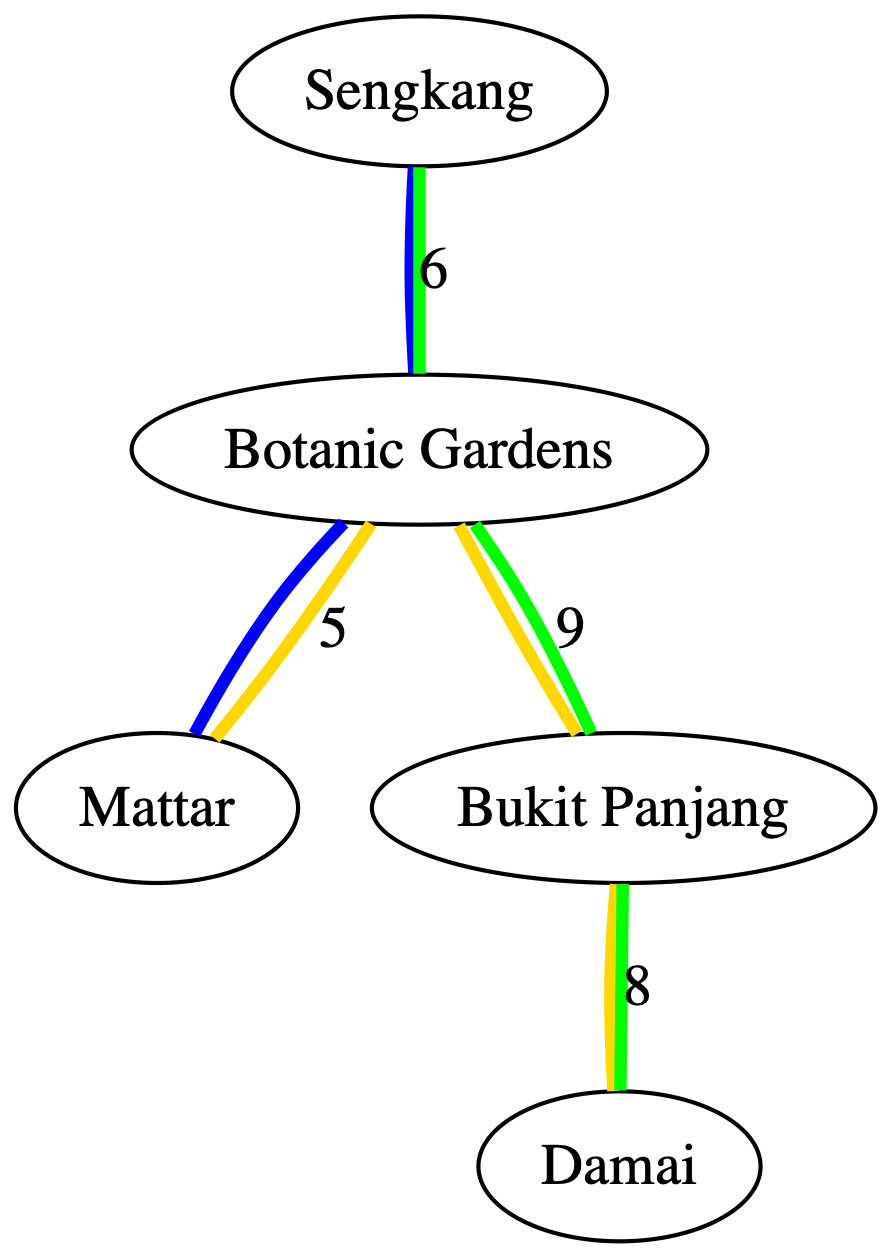
\includegraphics[width=\linewidth]{map}
		\captionof{figure}{Map of the train lines for 8 edges/trains}
	\end{minipage}
\end{center}
\newpage
\subsection{Raw Data Collected}
\begin{center}
	\begin{tabular}{r r r | r}
		num\_edge / num\_trains & num\_cores & short & time    \\
		\hline
		8                       & 8          & TRUE  & 1.152   \\
		8                       & 8          & FALSE & 1.229   \\
		8                       & 16         & TRUE  & 1.102   \\
		8                       & 16         & FALSE & 1.159   \\
		8                       & 32         & TRUE  & 1.177   \\
		8                       & 32         & FALSE & 1.260   \\
		8                       & NA         & TRUE  & 0.067   \\
		8                       & NA         & FALSE & 0.142   \\
		\hline
		16                      & 8          & TRUE  & 1.466   \\
		16                      & 8          & FALSE & 1.942   \\
		16                      & 16         & TRUE  & 10.216  \\
		16                      & 16         & FALSE & 10.270  \\
		16                      & 32         & TRUE  & 12.080  \\
		16                      & 32         & FALSE & 12.336  \\
		16                      & NA         & TRUE  & 0.076   \\
		16                      & NA         & FALSE & 0.289   \\
		\hline
		32                      & 8          & TRUE  & 2.004   \\
		32                      & 8          & FALSE & 2.459   \\
		32                      & 16         & TRUE  & 12.244  \\
		32                      & 16         & FALSE & 12.293  \\
		32                      & 32         & TRUE  & 15.611  \\
		32                      & 32         & FALSE & 15.843  \\
		32                      & NA         & TRUE  & 1.197   \\
		32                      & NA         & FALSE & 3.621   \\
		\hline
		64                      & 8          & TRUE  & 3.640   \\
		64                      & 8          & FALSE & 5.306   \\
		64                      & 16         & TRUE  & 382.949 \\
		64                      & 16         & FALSE & 470.589 \\
		64                      & 32         & TRUE  & 39.227  \\
		64                      & 32         & FALSE & 46.471  \\
		64                      & NA         & TRUE  & 2.772   \\
		64                      & NA         & FALSE & 8.345   \\
	\end{tabular}
	\captionof{table}{Data collected}
\end{center}

\section{Discussion}
It can be observed that the wall clock time taken for the simulation to complete increases as number of threads increases. This is because as number of threads increases, there is more contention of resources -- in our case contention for each train (thread) in using links (edges) between stations (vertices) and contention for each train in opening door at each station. We are managing this using an implicit queue through implementing a timekeeper to track the next allowed event to occur, protected by marking that section as critical. As such, for each link (edge) or station (vertex), only one train (thread) is able to register itself to the timekeeper at any given time -- others will have to wait.

However, we have an interesting observation as well. Notice that the execution time behaves very differently when the number of threads is beyond the number of logical cores (20 cores). For small input size (100 ticks), when the number of threads is beyond the number of logical cores, the execution time actually falls. However, as input size gets larger (1,000 and 10,000 ticks), execution time increases. This can be explained that when the number of threads are below the number of logical cores, all the threads are running concurrently, resulting in more lock contention (not to be confused with resource contention). However, when number of threads is above the number of logical cores, the threads take turns to wake up and do work, resulting in less lock contention. For smaller input size, the lock contention time actually outweighs the execution time, resulting in the fall in execution time. However, for larger input size, there is a large overhead in context-switching which outweighs the effect of lock contention time. This is supported by the data we collected on number of context-switches for 100 ticks and 1,000 ticks.

We also observe another trend -- that the variance in execution time falls when the number of threads exceed the number of logical cores. We currently have no explanation on this, but we suspect that the compiler does an optimisation when the number of threads exceed the number of logical cores.

% \newpage
% \begin{center}
% 	\captionof{figure}{Number of context switches for 100 ticks}
% 	\includegraphics[width=0.9\linewidth]{100-cs}
% \end{center}
% \begin{center}
% 	\captionof{figure}{Number of context switches for 1,000 ticks}
% 	\includegraphics[width=0.9\linewidth]{1000-cs}
% \end{center}

\section{Bonus}
Starvation will never occur in the simulation program that we wrote. This is because to decide which train to open door or to be allowed to use a link next, we are using a queue to implement First-Come-First-Serve (FCFS) scheduler, or in the case of the train doors, an implicit queue through the timekeeper. As such, every train is assured access to the link or permission to open door after a long enough time. The assumptions are that no train open its doors or travel using the links indefinitely (which we believe are fair to make).

\newpage
\section{Appendix A: Ruby script used to generate test cases}
Below is the code listing of the ruby script used to generate test cases. Essentially, it does:
\begin{enumerate}
	\item Create a random adjacency matrix with diagonal = 0
	\item Find the MST of the random graph created
	\item Ensure that there are enough vertices with degree = 1, else go back to step 1
	\item Enumerate the 2-combinations of the vertices with degree = 1, and pick 3 randomly.
	\item For each of the three 2-combinations, assign them to be the termini of each line.
	\item Using breadth-first-search, find the path between the two vertices for each pair of termini.
	\item Ensure that the path is long enough, else go back to step 4.
\end{enumerate}
\begin{minted}{Ruby}

  # SOME CODE

	\end{minted}
\end{document}
